\title{Web-Based Supporting Materials for\\
	``RNN-Based Counterfactual Prediction'' by Jason Poulos}

\date{}

%%%%%%%%%%%%%%%%%%%%%%%%%%%%%%%%%%%%%%%%%%%%%%%%%%
% Set document class
\documentclass[12pt]{article}

% Define packages
\usepackage{hyperref, url} 
\usepackage{graphicx,amsfonts,psfrag,layout,subcaption,array,longtable,lscape,booktabs,dcolumn,amsmath,amssymb,amssymb,amsthm,setspace,epigraph,chronology,color,colortbl,caption,wasysym,diagbox,natbib,colortbl}
\usepackage[]{graphicx}\usepackage[]{color}
\usepackage[page]{appendix}
\usepackage[section]{placeins}
\usepackage[linewidth=1pt]{mdframed}
\usepackage[margin={1in}]{geometry} %1 inch margins

%% Reference labels in the online appendix
\usepackage{xr}
\externaldocument{rnns-causal}

% Footnotes stick at the bottom
\usepackage[bottom]{footmisc}

% Caption keys
\usepackage{mathtools,tikz,caption}
\captionsetup{labelfont=sc,labelsep=period}
\DeclareRobustCommand\sampleline[1]{%
	\tikz\draw[#1] (0,0) (0,\the\dimexpr\fontdimen22\textfont2\relax)
	-- (2em,\the\dimexpr\fontdimen22\textfont2\relax);%
}

\usetikzlibrary{plotmarks}

% Wes Anderson colors

\usepackage{xcolor}

\definecolor{Darjeeling11}{HTML}{FF0000}
\definecolor{Darjeeling15}{HTML}{5BBCD6}

% New footnote characters
\usepackage{footmisc}
\DefineFNsymbols{mySymbols}{{\ensuremath\dagger}{\ensuremath\ddagger}\S\P
	*{**}{\ensuremath{\dagger\dagger}}{\ensuremath{\ddagger\ddagger}}}
\setfnsymbol{mySymbols}

% New tabular environment
\usepackage{tabularx}
\newcolumntype{Y}{>{\raggedleft\arraybackslash}X}% raggedleft column X

% Define appendix 
\renewcommand*\appendixpagename{Appendix}
\renewcommand*\appendixtocname{Appendix}

% Position floats
\renewcommand{\textfraction}{0.05}
\renewcommand{\topfraction}{0.95}
\renewcommand{\bottomfraction}{0.95}
\renewcommand{\floatpagefraction}{0.35}
\setcounter{totalnumber}{5}

% Colors for highlighting tables
\definecolor{Gray}{gray}{0.9}

% Different font in captions
\newcommand{\captionfonts}{\normalsize}

\makeatletter  % Allow the use of @ in command names
\long\def\@makecaption#1#2{%
	\vskip\abovecaptionskip
	\sbox\@tempboxa{{\captionfonts #1: #2}}%
	\ifdim \wd\@tempboxa >\hsize
	{\captionfonts #1: #2\par}
	\else
	\hbox to\hsize{\hfil\box\@tempboxa\hfil}%
	\fi
	\vskip\belowcaptionskip}
%\makeatother   % Cancel the effect of \makeatletter

% Set Spacing
%\singlespacing
%\doublespacing

% Number assumptions
\newtheorem*{assumption*}{\assumptionnumber}
\providecommand{\assumptionnumber}{}
\makeatletter
\newenvironment{assumption}[2]
{%
	\renewcommand{\assumptionnumber}{Assumption #1}%
	\begin{assumption*}%
		\protected@edef\@currentlabel{#1}%
	}
	{%
	\end{assumption*}
}
\makeatother

% Macros
\newcommand{\Adv}{{\mathbf{Adv}}}       
\newcommand{\prp}{{\mathrm{prp}}}                  % How to define new commands 
\newcommand{\calK}{{\cal K}}
\newcommand{\outputs}{{\Rightarrow}}                
\newcommand{\getsr}{{\:\stackrel{{\scriptscriptstyle\hspace{0.2em}\$}}{\leftarrow}\:}}
\newcommand{\andthen}{{\::\;\;}}    %  \: \; for thinspace, medspace, thickspace
\newcommand{\Rand}[1]{{\mathrm{Rand}[{#1}]}}       % A command with one argument
\newcommand{\Perm}[1]{{\mathrm{Perm}[{#1}]}}       
\newcommand{\Randd}[2]{{\mathrm{Rand}[{#1},{#2}]}} % and with two arguments
\newcommand{\E}{\mathrm{E}}
\newcommand{\Var}{\mathrm{Var}}
\newcommand{\Cov}{\mathrm{Cov}}
\DeclareMathOperator*{\plim}{plim}
\newcommand\independent{\protect\mathpalette{\protect\independenT}{\perp}}
\def\independenT#1#2{\mathrel{\rlap{$#1#2$}\mkern2mu{#1#2}}}
\newcommand{\possessivecite}[1]{\citeauthor{#1}'s [\citeyear{#1}]} 

\renewcommand*\contentsname{Table of contents}

%%%%%%%%%%%%%%%%%%%%%%%%%%%%%%%%%%%%%%%%%%%%%%%%%%%%%%%%%%%%%%%%%%%%%%%%%%%%

\begin{document}

\begin{singlespacing}
\maketitle \thispagestyle{empty}
\tableofcontents \thispagestyle{empty}
\end{singlespacing}

\pagenumbering{roman}% Roman-numbered pages (start from i)

\pagebreak
\pagenumbering{arabic}% Arabic-numbered pages (start from 1)

\section{RNNs architecture} 

\begin{figure}[htb]
	\begin{center}
		\includegraphics[width=0.5\textwidth]{/media/jason/Dropbox/github/rnns-causal/results/plots/encoder-decoder.png} \\
		\caption{Encoder-decoder networks architecture. Dropout is applied to the visible input sequences, which are then fed to a two-layer bidirectional LSTM encoder. The encoder encodes the input sequences into a single vector that contains information about the entire sequence. The output of the encoder is repeated $t$ times and fed to the single-layer GRU decoder, which translates the encoded sequence into the predicted sequence. Finally, a dense layer is applied to the decoder output to generate predictions. \label{encoder-decoder}} 
	\end{center}
\end{figure}

\begin{figure}[htbp]
	\begin{center}
		\includegraphics[width=0.5\textwidth]{/media/jason/Dropbox/github/gans-causal/results/plots/vae.png} \\
		\caption{Recurrent VAE architecture. First, an LSTM encoder turns the input samples into two parameters in a latent space. Latent space points are randomly sampled from the latent distribution that is assumed to generate the data. The sampling output is repeated $t$ times and fed to the decoder LSTM, which maps the latent space points back to the original input data.  \label{vae}} 
	\end{center}
\end{figure}

\section{Descriptive statistics}


\begin{figure*}[htbp]
	\centering
	\begin{subfigure}[t]{0.45\textwidth}
		\centering
		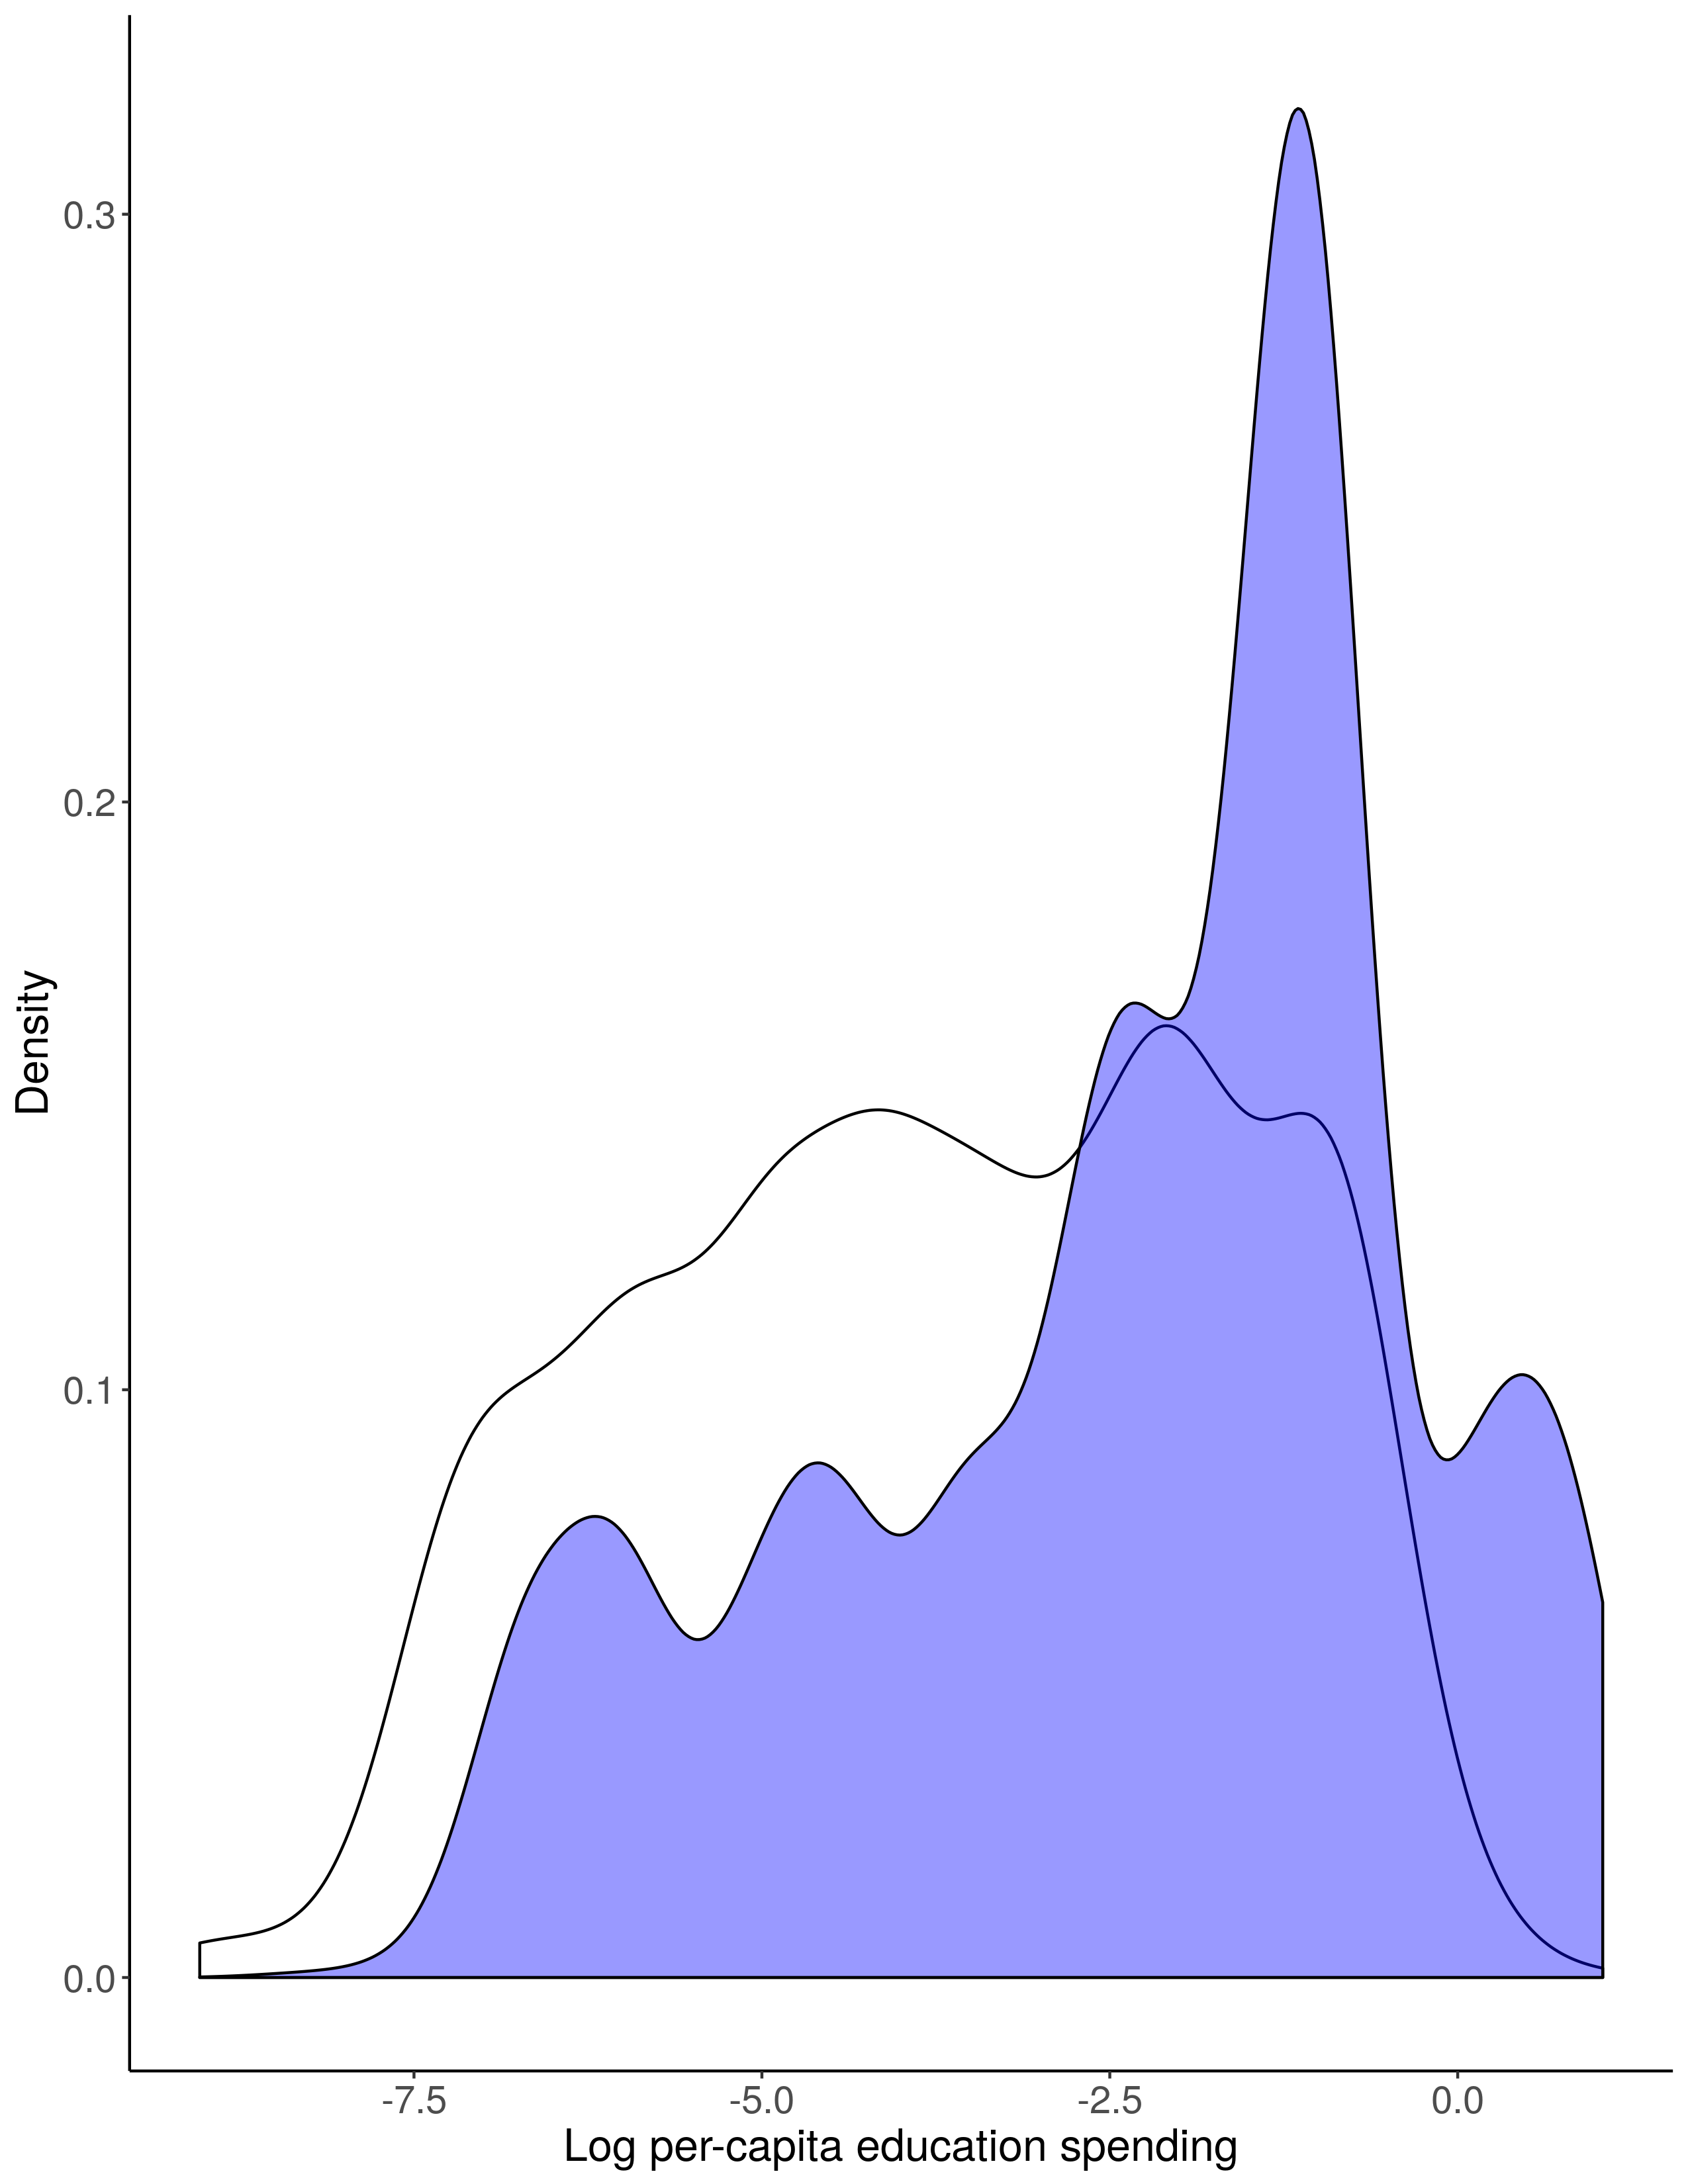
\includegraphics[width=\textwidth]{/media/jason/Dropbox/github/rnns-causal/results/plots/educ-dens.png}
		\caption{Unweighted \label{educ-dense}} 
	\end{subfigure}
	~ 
	\begin{subfigure}[t]{0.45\textwidth}
		\centering
		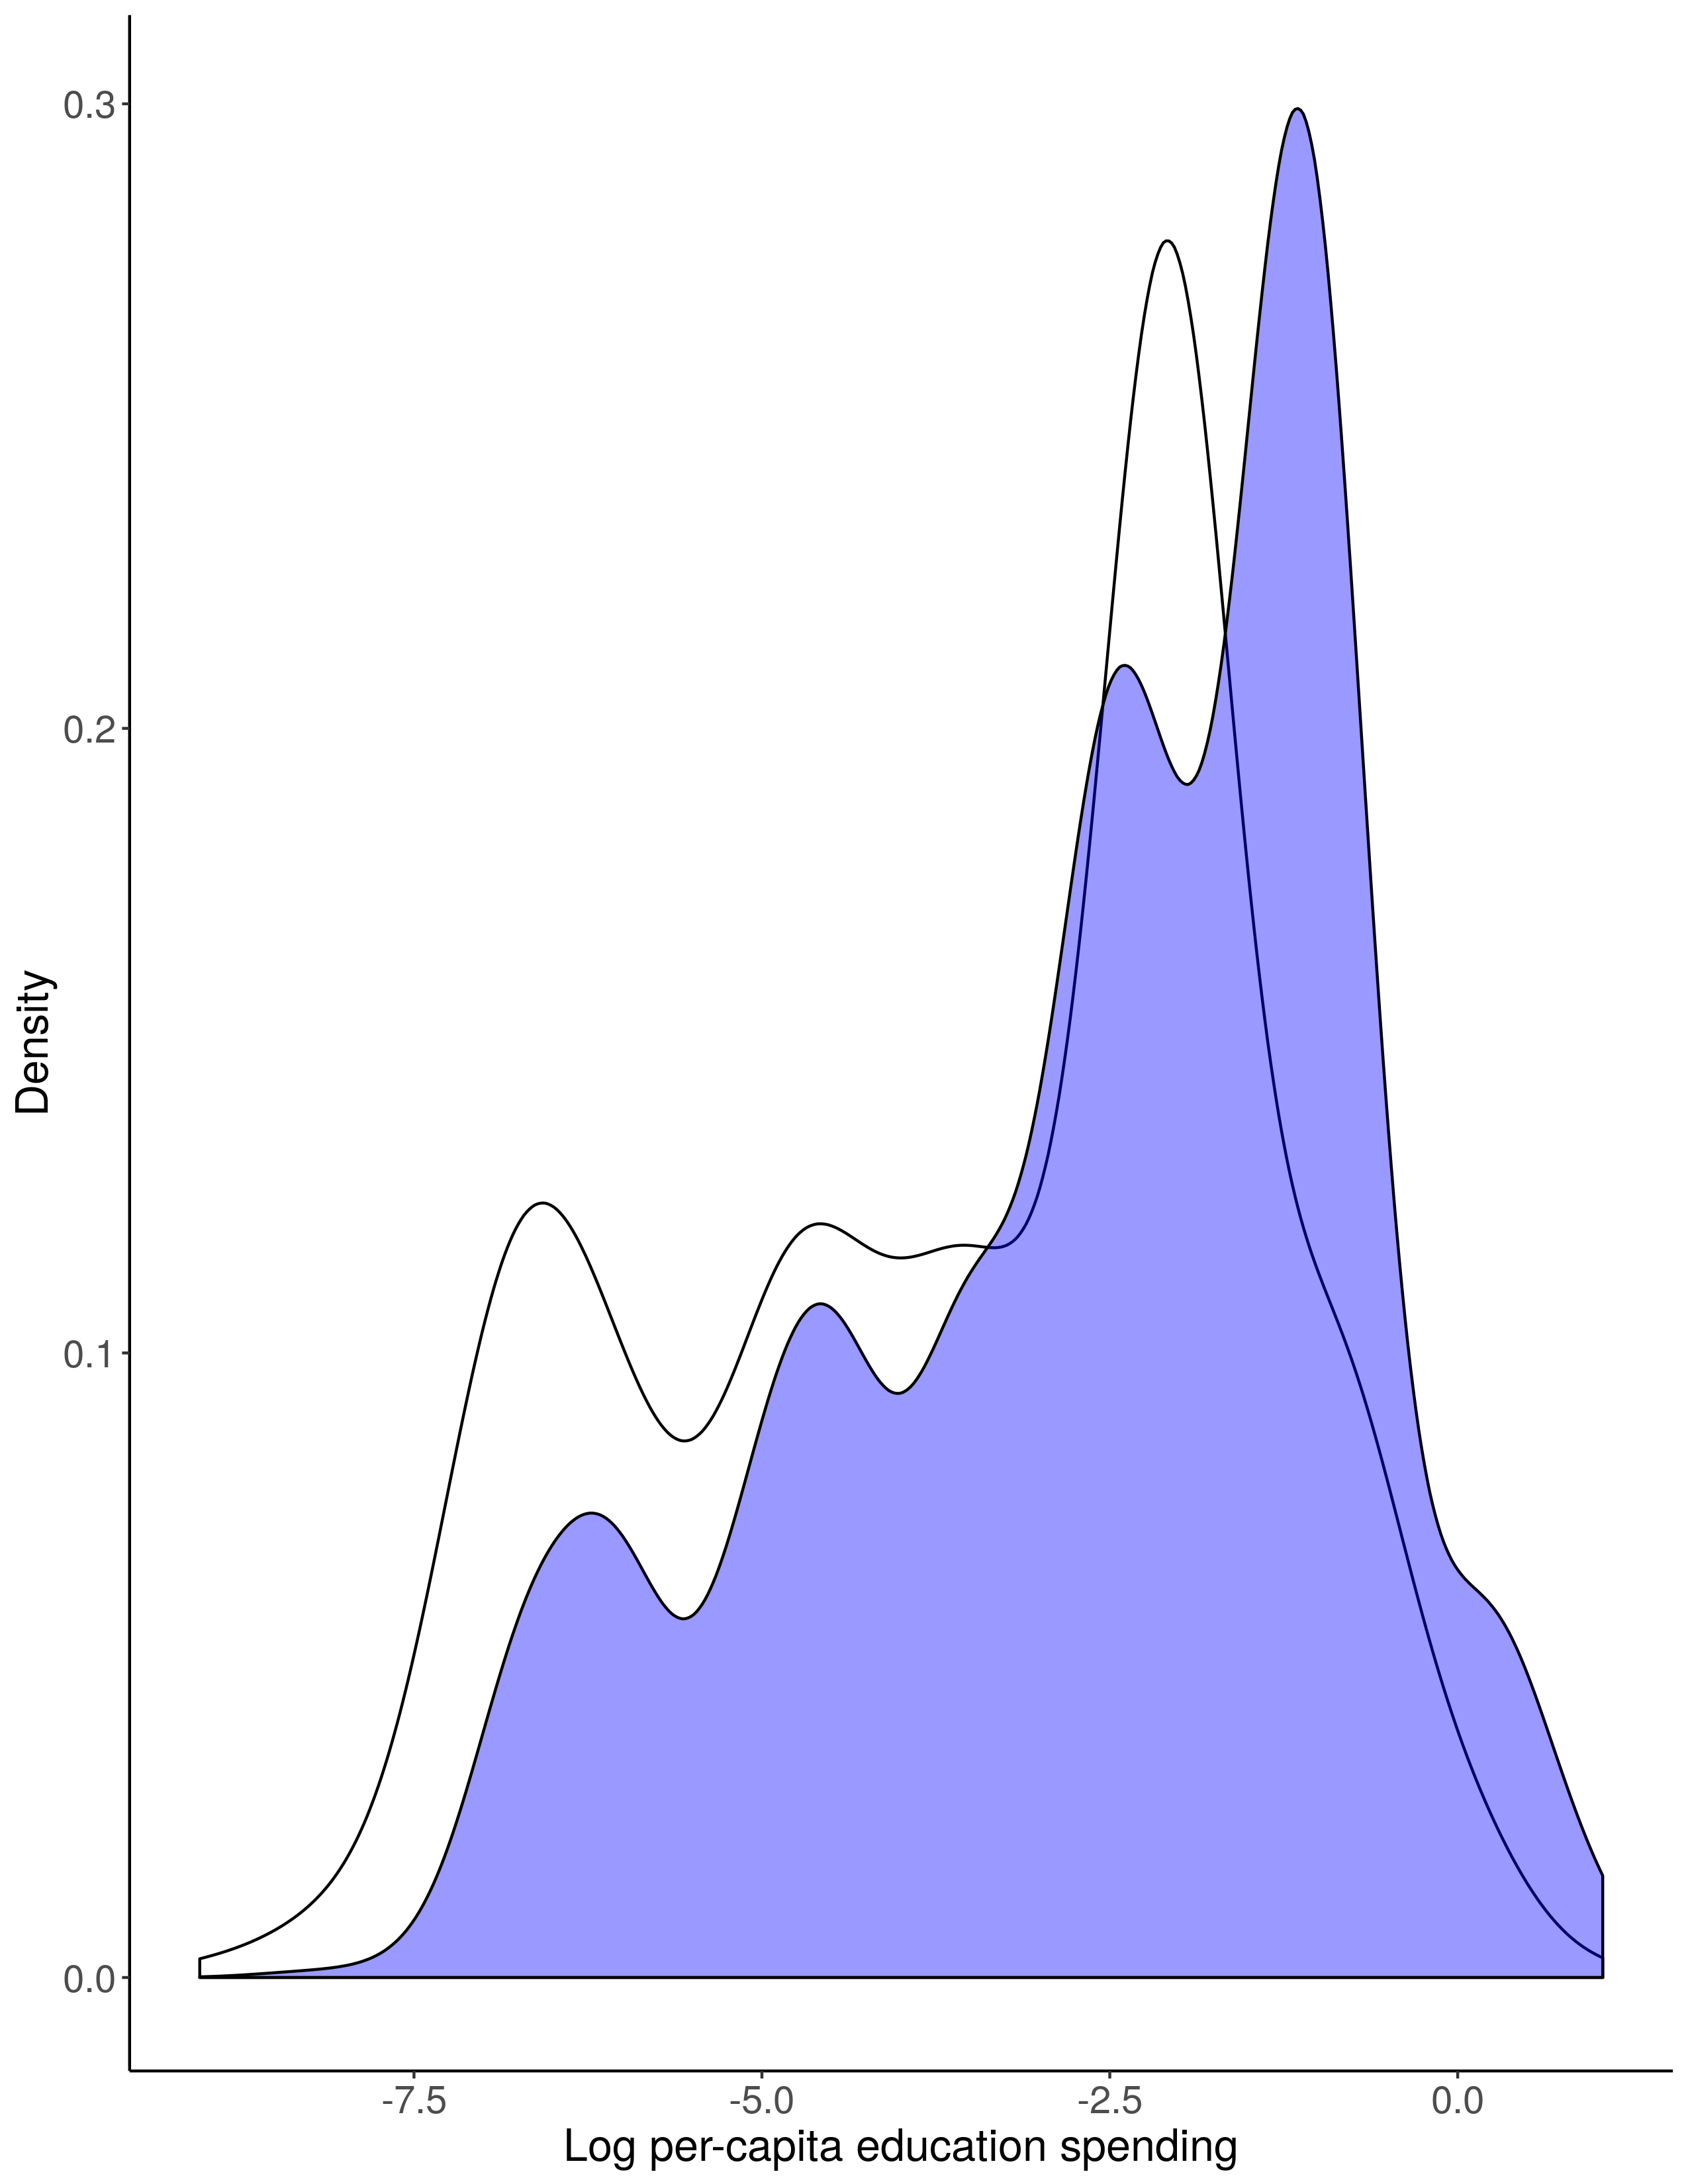
\includegraphics[width=\textwidth]{/media/jason/Dropbox/github/rnns-causal/results/plots/educ-dens-w.png}
		\caption{Weighted\label{educ-dense-w}}
	\end{subfigure}
	\caption{Pre-period densities of log per-capita state government education spending by treatment status. Density in \ref{educ-dense-w} weighted by propensity score.} 
\end{figure*}

\begin{figure}[htbp]
	\begin{center}
		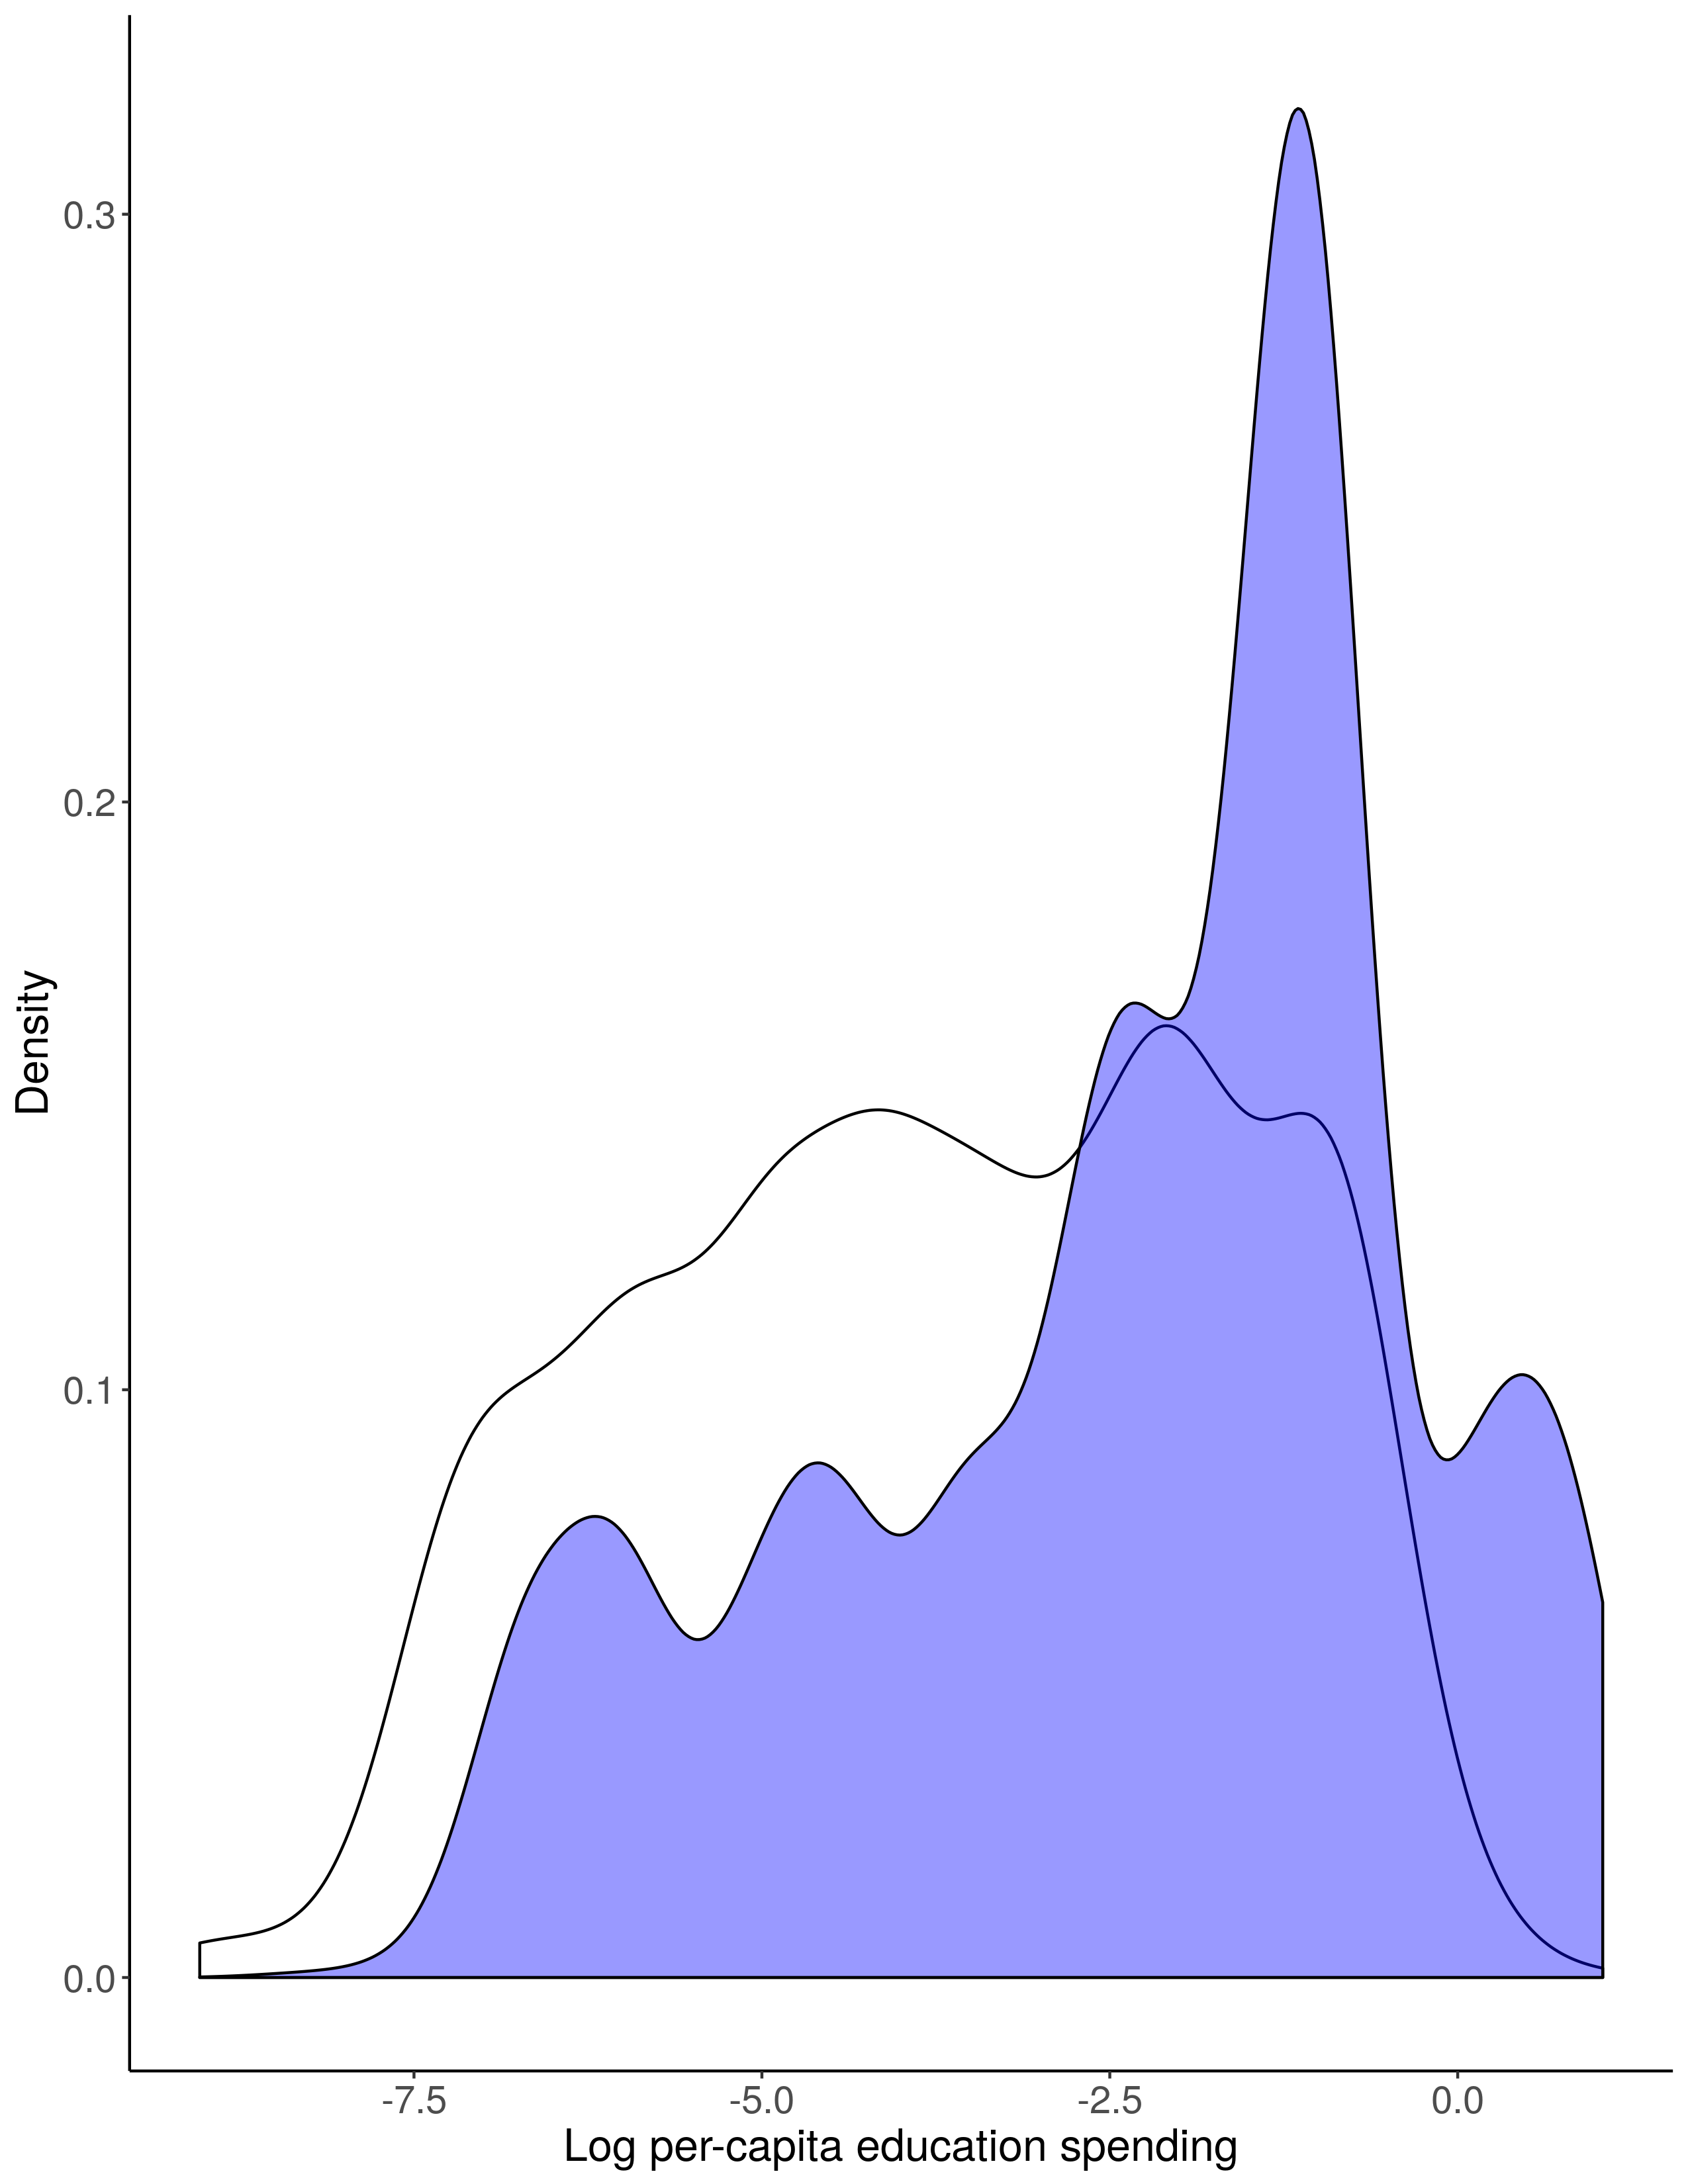
\includegraphics[width=0.8\textwidth]{/media/jason/Dropbox/github/rnns-causal/results/plots/educ-dens.png} \\
		\caption{(Left) Pre-period unweighted densities of log per-capita state government education spending by treatment status. (Right)  \label{educ-dense}} 
	\end{center}
\end{figure}

\section{RNNs training history: SCM datasets}

\begin{figure*}[htbp]
    \centering
    \begin{subfigure}[t]{0.4\textwidth}
        \centering
        \includegraphics[width=\textwidth]{/media/jason/Dropbox/github/rnns-causal/results/plots/encoder-decoder-basque-treated-loss.png}
        \caption{Basque Country (treated) \label{encoder-decoder-loss-basque-treated}} 
    \end{subfigure}
    ~ 
        \begin{subfigure}[t]{0.4\textwidth}
        \centering
        \includegraphics[width=\textwidth]{/media/jason/Dropbox/github/rnns-causal/results/plots/encoder-decoder-basque-control-loss.png}
        \caption{Basque Country (controls)}
    \end{subfigure}
    ~ %
    \begin{subfigure}[t]{0.4\textwidth}
        \centering
        \includegraphics[width=\textwidth]{/media/jason/Dropbox/github/rnns-causal/results/plots/encoder-decoder-california-treated-loss.png}
        \caption{California (treated)}
    \end{subfigure}
            ~ 
    \begin{subfigure}[t]{0.4\textwidth}
        \centering
        \includegraphics[width=\textwidth]{/media/jason/Dropbox/github/rnns-causal/results/plots/encoder-decoder-california-control-loss.png}
        \caption{California (controls)}
    \end{subfigure}
            ~ %
    \begin{subfigure}[t]{0.4\textwidth}
        \centering
        \includegraphics[width=\textwidth]{/media/jason/Dropbox/github/rnns-causal/results/plots/encoder-decoder-germany-treated-loss.png}
        \caption{West Germany (treated)}
    \end{subfigure}
            ~ 
    \begin{subfigure}[t]{0.4\textwidth}
        \centering
        \includegraphics[width=\textwidth]{/media/jason/Dropbox/github/rnns-causal/results/plots/encoder-decoder-germany-control-loss.png}
        \caption{West Germany (controls)}
    \end{subfigure}
\caption{Evolution of encoder-decoder networks training and validation loss in terms of MSPE. \label{encoder-decoder-loss-scm}} 
\end{figure*}

\begin{figure*}[htbp]
    \centering
    \begin{subfigure}[t]{0.4\textwidth}
        \centering
        \includegraphics[width=\textwidth]{/media/jason/Dropbox/github/rnns-causal/results/plots/lstm-basque-treated-loss.png}
        \caption{Basque Country (treated)}
    \end{subfigure}
    ~ 
        \begin{subfigure}[t]{0.4\textwidth}
        \centering
        \includegraphics[width=\textwidth]{/media/jason/Dropbox/github/rnns-causal/results/plots/lstm-basque-control-loss.png}
        \caption{Basque Country (controls)}
    \end{subfigure}
    ~ %
    \begin{subfigure}[t]{0.4\textwidth}
        \centering
        \includegraphics[width=\textwidth]{/media/jason/Dropbox/github/rnns-causal/results/plots/lstm-california-treated-loss.png}
        \caption{California (treated)}
    \end{subfigure}
            ~ 
                \begin{subfigure}[t]{0.4\textwidth}
        \centering
        \includegraphics[width=\textwidth]{/media/jason/Dropbox/github/rnns-causal/results/plots/lstm-california-control-loss.png}
        \caption{California (controls)}
    \end{subfigure}
            ~ %
    \begin{subfigure}[t]{0.4\textwidth}
        \centering
        \includegraphics[width=\textwidth]{/media/jason/Dropbox/github/rnns-causal/results/plots/lstm-germany-treated-loss.png}
        \caption{West Germany (treated)}
    \end{subfigure}
            ~ 
    \begin{subfigure}[t]{0.4\textwidth}
        \centering
        \includegraphics[width=\textwidth]{/media/jason/Dropbox/github/rnns-causal/results/plots/lstm-germany-control-loss.png}
        \caption{West Germany (controls)}
    \end{subfigure}
\caption{Evolution of baseline LSTM training and validation loss in terms of MSPE. \label{lstm-loss-scm}} 
\end{figure*}

\begin{figure*}[htbp]
	\centering
	\begin{subfigure}[t]{0.4\textwidth}
		\centering
		\includegraphics[width=\textwidth]{/media/jason/Dropbox/github/land-reform/results/plots/vae-basque-loss-treated.png}
		\caption{Basque Country (treated)}
	\end{subfigure}
	~ 
	\begin{subfigure}[t]{0.4\textwidth}
		\centering
		\includegraphics[width=\textwidth]{/media/jason/Dropbox/github/land-reform/results/plots/vae-basque-loss-control.png}
		\caption{Basque Country (controls)}
	\end{subfigure}
	~ %
	\begin{subfigure}[t]{0.4\textwidth}
		\centering
		\includegraphics[width=\textwidth]{/media/jason/Dropbox/github/land-reform/results/plots/vae-california-loss-treated.png}
		\caption{California (treated)}
	\end{subfigure}
	~ 
	\begin{subfigure}[t]{0.4\textwidth}
		\centering
		\includegraphics[width=\textwidth]{/media/jason/Dropbox/github/land-reform/results/plots/vae-california-loss-control.png}
		\caption{California (controls)}
	\end{subfigure}
	~ %
	\begin{subfigure}[t]{0.4\textwidth}
		\centering
		\includegraphics[width=\textwidth]{/media/jason/Dropbox/github/land-reform/results/plots/vae-germany-loss-treated.png}
		\caption{West Germany (treated)}
	\end{subfigure}
	~ 
	\begin{subfigure}[t]{0.4\textwidth}
		\centering
		\includegraphics[width=\textwidth]{/media/jason/Dropbox/github/land-reform/results/plots/vae-germany-loss-control.png}
		\caption{West Germany (controls)}
	\end{subfigure}
	\caption{Evolution of VAE training and validation loss in terms of MSPE. \label{vae-loss-scm}} 
\end{figure*}

\section{Estimates on Basque Country data}

\begin{figure*}[htbp] % treated time-series plots 
    \centering
    \begin{subfigure}[t]{0.5\textwidth}
        \centering
        \includegraphics[width=\textwidth]{/media/jason/Dropbox/github/rnns-causal/results/plots/encoder-decoder-plot-basque.png}
        \caption{Encoder-decoder}
    \end{subfigure}%
        ~ 
    \begin{subfigure}[t]{0.5\textwidth}
        \centering
        \includegraphics[width=\textwidth]{/media/jason/Dropbox/github/rnns-causal/results/plots/lstm-plot-basque.png}
        \caption{LSTM (baseline)}
    \end{subfigure}
        ~ 
    \begin{subfigure}[t]{0.5\textwidth}
        \centering
        \includegraphics[width=\textwidth]{/media/jason/Dropbox/github/rnns-causal/results/plots/synth-plot-predictions-basque.png}
        \caption{SCM}
    \end{subfigure}%
        ~ 
    \begin{subfigure}[t]{0.5\textwidth}
		\centering
		\includegraphics[width=\textwidth]{/media/jason/Dropbox/github/land-reform/results/plots/vae-plot-basque.png}
		\caption{VAE}
	\end{subfigure}
    \caption{Observed and counterfactual predicted outcomes for treated unit in Basque Country dataset.\label{basque-plot}}
\end{figure*}

\begin{figure*}[htbp]
	\centering
	\begin{subfigure}[t]{0.5\textwidth}
		\centering
		\includegraphics[width=\textwidth]{/media/jason/Dropbox/github/rnns-causal/results/plots/encoder-decoder-plot-effects-basque.png}
		\caption{Encoder-decoder}
	\end{subfigure}%
	~ 
	\begin{subfigure}[t]{0.5\textwidth}
		\centering
		\includegraphics[width=\textwidth]{/media/jason/Dropbox/github/rnns-causal/results/plots/lstm-plot-effects-basque.png}
		\caption{LSTM}
	\end{subfigure}
	~ 
	\begin{subfigure}[t]{0.5\textwidth}
		\centering
		\includegraphics[width=\textwidth]{/media/jason/Dropbox/github/rnns-causal/results/plots/synth-plot-basque.png}
		\caption{SCM}
	\end{subfigure}%
	~ 
	\begin{subfigure}[t]{0.5\textwidth}
		\centering
		\includegraphics[width=\textwidth]{/media/jason/Dropbox/github/land-reform/results/plots/vae-plot-effects-basque.png}
		\caption{VAE}
	\end{subfigure}
	\caption{Time-series of post-period treatment effects in Basque Country dataset. Darker line represents the effect on the actual treated unit and each lighter line represents the effects on control units. Shaded regions represent 95\% randomization confidence intervals. \label{basque-plot-effects}}
\end{figure*}

\begin{figure*}[htbp]
    \centering
    \begin{subfigure}[t]{0.5\textwidth}
        \centering
        \includegraphics[width=\textwidth]{/media/jason/Dropbox/github/rnns-causal/results/plots/encoder-decoder-plot-pvalues-basque.png}
        \caption{Encoder-decoder}
    \end{subfigure}%
        ~ 
    \begin{subfigure}[t]{0.5\textwidth}
        \centering
        \includegraphics[width=\textwidth]{/media/jason/Dropbox/github/rnns-causal/results/plots/lstm-plot-pvalues-basque.png}
        \caption{LSTM (baseline)}
    \end{subfigure}
        ~ 
    \begin{subfigure}[t]{0.5\textwidth}
        \centering
        \includegraphics[width=\textwidth]{/media/jason/Dropbox/github/rnns-causal/results/plots/synth-plot-pvalues-basque.png}
        \caption{SCM}
     \end{subfigure}%
                ~ 
     \begin{subfigure}[t]{0.5\textwidth}
       	\centering
       	\includegraphics[width=\textwidth]{/media/jason/Dropbox/github/land-reform/results/plots/vae-plot-pvalues-basque.png}
       	\caption{VAE}
    \end{subfigure}
    \caption{Per-period randomization $p$-values corresponding to treatment effects on treated and control units in Basque Country dataset. \label{basque-plot-pvalues}}
\end{figure*}

\section{Estimates on California data}

\begin{figure*}[htbp] % treated time-series plots 
    \centering
    \begin{subfigure}[t]{0.5\textwidth}
        \centering
        \includegraphics[width=\textwidth]{/media/jason/Dropbox/github/rnns-causal/results/plots/encoder-decoder-plot-california.png}
        \caption{Encoder-decoder}
    \end{subfigure}%
        ~ 
    \begin{subfigure}[t]{0.5\textwidth}
        \centering
        \includegraphics[width=\textwidth]{/media/jason/Dropbox/github/rnns-causal/results/plots/lstm-plot-california.png}
        \caption{LSTM (baseline)}
    \end{subfigure}
        ~ 
    \begin{subfigure}[t]{0.5\textwidth}
        \centering
        \includegraphics[width=\textwidth]{/media/jason/Dropbox/github/rnns-causal/results/plots/synth-plot-predictions-california.png}
        \caption{SCM}
    \end{subfigure}%
         ~ 
	\begin{subfigure}[t]{0.5\textwidth}
		\centering
		\includegraphics[width=\textwidth]{/media/jason/Dropbox/github/land-reform/results/plots/vae-plot-california.png}
		\caption{VAE}
	\end{subfigure}
    \caption{Observed and counterfactual predicted outcomes for treated unit in California dataset.\label{california-plot}}
\end{figure*}

\begin{figure*}[htbp]
	\centering
	\begin{subfigure}[t]{0.5\textwidth}
		\centering
		\includegraphics[width=\textwidth]{/media/jason/Dropbox/github/rnns-causal/results/plots/encoder-decoder-plot-effects-california.png}
		\caption{Encoder-decoder}
	\end{subfigure}%
	~ 
	\begin{subfigure}[t]{0.5\textwidth}
		\centering
		\includegraphics[width=\textwidth]{/media/jason/Dropbox/github/rnns-causal/results/plots/lstm-plot-effects-california.png}
		\caption{LSTM}
	\end{subfigure}
	~ 
	\begin{subfigure}[t]{0.5\textwidth}
		\centering
		\includegraphics[width=\textwidth]{/media/jason/Dropbox/github/rnns-causal/results/plots/synth-plot-california.png}
		\caption{SCM}
	\end{subfigure}%
	~ 
	\begin{subfigure}[t]{0.5\textwidth}
		\centering
		\includegraphics[width=\textwidth]{/media/jason/Dropbox/github/land-reform/results/plots/vae-plot-effects-california.png}
		\caption{VAE}
	\end{subfigure}
	\caption{Time-series of post-period treatment effects in California dataset. See notes to SM-Fig. \ref{basque-plot-effects}.\label{california-plot-effects}}
\end{figure*}

\begin{figure*}[htbp]
    \centering
    \begin{subfigure}[t]{0.5\textwidth}
        \centering
        \includegraphics[width=\textwidth]{/media/jason/Dropbox/github/rnns-causal/results/plots/encoder-decoder-plot-pvalues-california.png}
        \caption{Encoder-decoder}
    \end{subfigure}%
        ~ 
    \begin{subfigure}[t]{0.5\textwidth}
        \centering
        \includegraphics[width=\textwidth]{/media/jason/Dropbox/github/rnns-causal/results/plots/lstm-plot-pvalues-california.png}
        \caption{LSTM (baseline)}
    \end{subfigure}
        ~ 
    \begin{subfigure}[t]{0.5\textwidth}
        \centering
        \includegraphics[width=\textwidth]{/media/jason/Dropbox/github/rnns-causal/results/plots/synth-plot-pvalues-california.png}
        \caption{SCM}
    \end{subfigure}%
         ~ 
	\begin{subfigure}[t]{0.5\textwidth}
		\centering
		\includegraphics[width=\textwidth]{/media/jason/Dropbox/github/land-reform/results/plots/vae-plot-pvalues-california.png}
		\caption{VAE}
	\end{subfigure}
    \caption{Per-period randomization $p$-values corresponding to treatment effects on treated and control units in California dataset. \label{california-plot-pvalues}}
\end{figure*}

\section{Estimates on West Germany data}

\begin{figure*}[htbp] % treated time-series plots 
    \centering
    \begin{subfigure}[t]{0.5\textwidth}
        \centering
        \includegraphics[width=\textwidth]{/media/jason/Dropbox/github/rnns-causal/results/plots/encoder-decoder-plot-germany.png}
        \caption{Encoder-decoder}
    \end{subfigure}%
        ~ 
    \begin{subfigure}[t]{0.5\textwidth}
        \centering
        \includegraphics[width=\textwidth]{/media/jason/Dropbox/github/rnns-causal/results/plots/lstm-plot-germany.png}
        \caption{LSTM (baseline)}
    \end{subfigure}
        ~ 
    \begin{subfigure}[t]{0.5\textwidth}
        \centering
        \includegraphics[width=\textwidth]{/media/jason/Dropbox/github/rnns-causal/results/plots/synth-plot-predictions-germany.png}
        \caption{SCM}
    \end{subfigure}%
        ~ 
	\begin{subfigure}[t]{0.5\textwidth}
		\centering
		\includegraphics[width=\textwidth]{/media/jason/Dropbox/github/land-reform/results/plots/vae-plot-germany.png}
		\caption{VAE}
	\end{subfigure}
    \caption{Observed and counterfactual predicted outcomes for treated unit in West Germany dataset.\label{germany-plot}}
\end{figure*}


\begin{figure*}[htbp]
	\centering
	\begin{subfigure}[t]{0.5\textwidth}
		\centering
		\includegraphics[width=\textwidth]{/media/jason/Dropbox/github/rnns-causal/results/plots/encoder-decoder-plot-effects-germany.png}
		\caption{Encoder-decoder}
	\end{subfigure}%
	~ 
	\begin{subfigure}[t]{0.5\textwidth}
		\centering
		\includegraphics[width=\textwidth]{/media/jason/Dropbox/github/rnns-causal/results/plots/lstm-plot-effects-germany.png}
		\caption{LSTM}
	\end{subfigure}
	~ 
	\begin{subfigure}[t]{0.5\textwidth}
		\centering
		\includegraphics[width=\textwidth]{/media/jason/Dropbox/github/rnns-causal/results/plots/synth-plot-germany.png}
		\caption{SCM}
	\end{subfigure}%
	~ 
	\begin{subfigure}[t]{0.5\textwidth}
		\centering
		\includegraphics[width=\textwidth]{/media/jason/Dropbox/github/land-reform/results/plots/vae-plot-effects-germany.png}
		\caption{VAE}
	\end{subfigure}
	\caption{Time-series of post-period treatment effects in West Germany dataset. See notes to Fig. SM-\ref{basque-plot-effects}.\label{germany-plot-effects}}
\end{figure*}

\begin{figure*}[htbp]
    \centering
    \begin{subfigure}[t]{0.5\textwidth}
        \centering
        \includegraphics[width=\textwidth]{/media/jason/Dropbox/github/rnns-causal/results/plots/encoder-decoder-plot-pvalues-germany.png}
        \caption{Encoder-decoder}
    \end{subfigure}%
        ~ 
    \begin{subfigure}[t]{0.5\textwidth}
        \centering
        \includegraphics[width=\textwidth]{/media/jason/Dropbox/github/rnns-causal/results/plots/lstm-plot-pvalues-germany.png}
        \caption{LSTM (baseline)}
    \end{subfigure}
        ~ 
    \begin{subfigure}[t]{0.5\textwidth}
        \centering
        \includegraphics[width=\textwidth]{/media/jason/Dropbox/github/rnns-causal/results/plots/synth-plot-pvalues-germany.png}
        \caption{SCM}
    \end{subfigure}%
         ~ 
	\begin{subfigure}[t]{0.5\textwidth}
		\centering
		\includegraphics[width=\textwidth]{/media/jason/Dropbox/github/land-reform/results/plots/vae-plot-pvalues-germany.png}
		\caption{VAE}
	\end{subfigure}
    \caption{Per-period randomization $p$-values corresponding to treatment effects on treated and control units in West Germany dataset. \label{germany-plot-pvalues}}
\end{figure*}

\section{RNNs training history: Education spending data}

\begin{figure*}[htbp]
	\centering
	\begin{subfigure}[t]{0.45\textwidth}
		\centering
		\includegraphics[width=\textwidth]{/media/jason/Dropbox/github/land-reform/results/plots/encoder-decoder-west-educpc-loss-treated.png}
		\caption{Education Spending in West (treated)} 
	\end{subfigure}
	~ 
	\begin{subfigure}[t]{0.45\textwidth}
		\centering
		\includegraphics[width=\textwidth]{/media/jason/Dropbox/github/land-reform/results/plots/encoder-decoder-west-educpc-loss-control.png}
		\caption{Education Spending in West (controls)}
	\end{subfigure}
	\caption{Encoder-decoder networks training (solid line) and validation loss (dashed line). \label{encoder-decoder-loss-capacity-west}} 
\end{figure*}

\begin{figure*}[htbp]
	\centering
	\begin{subfigure}[t]{0.45\textwidth}
		\centering
		\includegraphics[width=\textwidth]{/media/jason/Dropbox/github/land-reform/results/plots/lstm-west-educpc-loss-treated.png}
		\caption{Education Spending in West (treated)} 
	\end{subfigure}
	~ 
	\begin{subfigure}[t]{0.45\textwidth}
		\centering
		\includegraphics[width=\textwidth]{/media/jason/Dropbox/github/land-reform/results/plots/lstm-west-educpc-loss-control.png}
		\caption{Education Spending in West (controls)}
	\end{subfigure}
	\caption{LSTM training (solid line) and validation loss (dashed line). \label{lstm-loss-capacity-west}} 
\end{figure*}

\section{Estimates on education spending data}

\begin{figure*}[htbp]
	\centering
	\includegraphics[width=\textwidth]{/media/jason/Dropbox/github/land-reform/results/plots/encoder-decoder-plot-west-educpc.png}
	\caption{Observed (solid line) and counterfactual predicted (dashed line) outcomes for treated unit. Dashed vertical line represents intervention year. \label{state-capacity-plot}}
\end{figure*}

\begin{figure*}[htbp]
		\centering
		\includegraphics[width=\textwidth]{/media/jason/Dropbox/github/land-reform/results/plots/encoder-decoder-plot-effects-west-educpc.png}
		\caption{Time-series of post-period treatment effects in state capacity datasets. Darker line represents the effect on the actual treated unit and each lighter line represents the effects on placebo treated units. Shaded regions represent 95\% randomization confidence intervals. \label{state-capacity-plot-effects}}
\end{figure*}

\begin{table}[htbp]
	\begin{center}
		\caption{Encoder-decoder FPR and MSPE on state capacity placebo tests.\label{encoder-decoder-mpse}}
		\resizebox{\width}{!}{\input{/media/jason/Dropbox/github/land-reform/unsourced-paper/encoder-decoder-mpse}} \\
		\footnotesize{Note: Errors represent $\pm$ one standard deviation from the MSPE.}
	\end{center}
\end{table}

\begin{table}[htbp]
	\begin{center}
		\caption{LSTM FPR and MSPE on state capacity placebo tests.\label{lstm-mpse}}
		\resizebox{\width}{!}{\input{/media/jason/Dropbox/github/land-reform/unsourced-paper/lstm-mpse}} \\
		\footnotesize{Note: Errors represent $\pm$ one standard deviation from the MSPE.}
	\end{center}
\end{table}

\begin{figure*}[htbp]
		\centering
		\includegraphics[width=\textwidth]{/media/jason/Dropbox/github/land-reform/results/plots/encoder-decoder-plot-pvalues-west-educpc.png}
	\caption{Encoder-decoder networks: Per-period randomization $p$-values corresponding to treatment effects on treated and control units in state capacity datasets. Darker dot represents $p$-values associated with treatment effects on the actual treated unit and lighter dots represent $p$-values associated with the effects on control units \label{state-capacity-plot-pvalues}}
\end{figure*}

\itemize
\end{document}
